%************************************************
\chapter{Design}\label{ch:design}
%************************************************

%************************************************
\section{Requirements} % (fold)
\label{sec:requirements}
%************************************************
In Section \ref{sec:goal} we have defined the main goals of the system as a list of high level system requirements. They are very generic and hard to establish an architecture upon. Because they do not contain details of the functionality the end-user of the system will be able to use. To have a clear vision of what this system needs to achieve, we will defined in this section a list of requirements from the end-user's perspective.\\

We have decided to use the user stories concept\cite{cohn2004user}, as a way to express the requirements of this system.\\

Agile Software Development is an iterative and incremental software development methodology, promoting adaptive planning, evolutionary development and delivery, while encouraging rapid and flexible response to change \cite{agile:online}. It is mainly used in the industry. One of the best practices in Agile Software Development for requirements is \emph{user stories}. We have not employed Agile Software Development in this work, but we have used the user stories concept as the agile methodology and the iterative design process resemble similarities and applying the user stories in this context, comes naturally.\\

''A user story describes functionality that will be valuable to either a user or purchaser of a system or software'' \cite{cohn2004user}. User stories are written from the perspective of the system's users. A specific group of users, will use the system in a certain way; the feature requested by this group represents a \emph{user role}. The user role does not necessarily have to be assigned to a human user; it can also be an external service in need of accessing some data.\\

%************************************************
\subsection{User Roles}\label{subsec:user_roles}
%************************************************
Writing the requirements following the user story concept, helps us reflect upon the needs this framework must satisfy, from the user's perspective. Based on the goals of the system defined in Section \ref{sec:goal} and supported by the use case scenario defined in Section \ref{sec:scenario}, we have first identified the user roles for this framework:
\begin{table}[H]
	\begin{center}
		\small \begin{tabular*}{1.1\columnwidth}{p{3cm}p{3cm}p{5.5cm}} 
			\\ \hline \hline
			Role & Who & Role Description \\ \hline \hline

		 	System Designer & The researcher & As discussed in the introduction \ref{ch:introduction}, someone designing a mobile context-aware system based on the egocentric interaction paradigm. Uses the framework to design a simulation of the egocentric system.\\ \hline

		 	Simulation User & The researcher, a QA engineer, an end-user of the egocentric system & This role can be fulfilled by users interested in the resulting egocentric system.\\ \hline

		 	Third Party Service & An individual piece of software & An individual piece of software that builds business logic based on the monitored context data, as the simulation unfolds.\\ \hline
		\end{tabular*}
		
		\caption{List of roles for the EgoSim framework}
		\label{table:roles}
	\end{center}
\end{table}
The ''who'' presents the possible user types that can fulfil a specific role, while the ''description'' briefly describes the role's main interest in the system.\\
% section user_roles (end)

%************************************************
\subsection{User Stories}\label{subsec:user_stories}
%************************************************
The following list of user stories, represent the requirements of the EgoSim framework:
\begin{enumerate}
	\item[\textlabel{1.}{us:1}] \emph{As a system designer, I want to model the environment my egocentric system will run in. The environment's model has to be populated with everyday physical objects and devices}. It is part of goal \ref{goal:1} and presented as a need in points \ref{scenario:1}, \ref{scenario:1A}, \ref{scenario:1B} and \ref{scenario:1C}.

	\item[\textlabel{2.}{us:2}] \emph{As a system designer, I need to identify the objects I want to be monitored during the simulation}, as described in goal \ref{goal:2} and point \ref{scenario:1D} in the scenario.

	\item[\textlabel{2.1}{us:2.1}] \emph{As a system designer, I want to specify how certain entities can be interacted with}. Points \ref{scenario:1E}, \ref{scenario:1F}, \ref{scenario:1G} and \ref{scenario:1H} illustrate a few ways entities could be interacted with.

	\item[\textlabel{2.2.}{us:2.2}] \emph{As a system designer, I want to augment objects that will be monitored with information needed by the SSM model}, as illustrated in point \ref{scenario:1I}. In order for the SSM classification to work, it needs to be aware of specific parameters for each entity. By default, each monitored entity will carry a set of default SSM configuration data, but certain entities might need some adjusted values. The SSM configuration parameters are detailed in Section \ref{subsec:ssm_params}.

	\item[\textlabel{3.}{us:3}] \emph{As a system designer, I want to run a simulation based on the environment model I have set up}.

	\item[\textlabel{4.}{us:4}] \emph{As a simulation user, I want to control a virtual avatar within the simulated environment}. This behaviour is mentioned in goal \ref{goal:1} and, as described in points \ref{scenario:2}, \ref{scenario:2A}, \ref{scenario:2B} and \ref{scenario:2C}, I want to be able to control the movement and field of vision of the agent. Also, I want to be able to pick up certain objects, carry them around and make them interact with other objects (e.g. put it down on a surface).

	\item[\textlabel{5.}{us:5}] \emph{As a simulation user, I want to have a sense of reality in the simulated environment}. The user should comprehend and fell present in the target environment.

	\item[\textlabel{6.}{us:6}] \emph{As a system designer, I want the simulation to classify monitored objects into SSM sets as the agent is being controlled}. This requirement is mentioned in goal \ref{goal:2} and highlighted in the scenario throughout points \ref{scenario:2D} and \ref{scenario:2E}. The SSM sets are detailed in Section \ref{subsec:ssm_params}.

	\item[\textlabel{7.}{us:7}] \emph{As a third party service, I want to access the content of SSM sets through a publicly available API from within the simulation}. Goal \ref{goal:3} covers this requirement, while point \ref{scenario:3} describes a useful scenario.

	\item[\textlabel{8.}{us:8}] \emph{As a simulation user, I want to follow the state of SSM sets, in real time, as the simulation unfolds}. As described in goal \ref{goal:3}, this requirement satisfies the need for an ''easy way to visualize the SSM spaces in real-time''.

\end{enumerate}

While an extra requirement is needed to fully support the situative space model - namely, representation of and interaction with virtual objects - we leave that requirement for future work.\\
% section user_stories (end)

%************************************************
\subsection{Non-functional Requirements}\label{subsec:nfrs}
%************************************************
To strengthen the requirements above, we conclude this section with a list of non-functional requirements (NFRs)\footnote{constraints on the system's behaviour}:
\begin{table}[H]
	\begin{center}
		\small \begin{tabular*}{1.1\columnwidth}{p{10cm}p{1.5cm}} 
			\\ \hline \hline
			NFR & Relates to \\ \hline \hline

		 	The agent should not be able to pass through walls and other objects in the environment. & \ref{us:4}\\ \hline

		 	The visualization of simulated environment should be non-blocking. No matter how heavy are the computations carried out under the hood, the simulation user's experience should not be affected. & \ref{us:5}\\ \hline

		 	Only objects within the field of vision of the user should be categorised & \ref{us:6}\\ \hline

		 	The SSM classification should happen in real-time. & \ref{us:6}\\ \hline

		\end{tabular*}
		
		\caption{Non functional requirements}
		\label{table:nfr}
	\end{center}
\end{table}
% section nfrs (end)

\subsection{SSM Sets and Configuration Parameters}\label{subsec:ssm_params}
In this work, we have focused on two main parameters to classify objects around the agent: proximity and field of vision. This means that objects within the agent's field of vision will be classified based on the distance from the agent's current position. We have given a less generic interpretation to the SSM Sets defined in \cite{pederson2011situative}, to fit this use case, as presented in the list below:
\paragraph{World Space} contains the set of all entities (physical objects and mediators) in the environment's virtual model. The framework takes into account only the entities which have been identified to be monitored. Hence, not all visible objects visible are categorized.
\paragraph{Perception Space} is part of space around the agent that is within the agent's field of vision at each moment. Objects within this space that are no further than \emph{PERCEPTION\_DISTANCE} from the agent, will be classified into this set.
\paragraph{Recognition Set} contains the entities that are currently in Perception Space and within their \emph{RECOGNITION\_DISTANCE}. Objects in this space can be directly associated with the agent's activities. For example, a hammer can be perceived as an object up to a certain distance, but when close enough, it can be recognised as a hammer.
\paragraph{Examinable Set} contains the objects that are currently in Perception Space and within their \emph{EXAMINATION\_DISTANCE}. Based on this set it can be determined what actions can be performed with that object. For example, in the perception space a cell phone can be seen as a simple object, in the recognizable set it can be recognized as a mobile device and in the examinable set one can notice it has a screen, a power button and two volume button. We can deduct the type of action one can perform!
\paragraph{Action Space} part of space around the agent that is currently accessible to the agent's physical actions. More specifically, the object has to currently be in Perception Space and within \emph{ACTION\_DISTANCE}. Objects in this set can be directly acted upon.
\paragraph{Selected Set} objects currently being physically handled.
\paragraph{Manipulated Set} objects whose states (external and internal) are currently being changed by the agent. Normally a subset of the Selected Set.\\

The image in Figure \ref{fig:req_ssm_sets} presents a graphical representation of the SSM to clarify the relationship between the sets.
\begin{figure}[H]
	\centering
	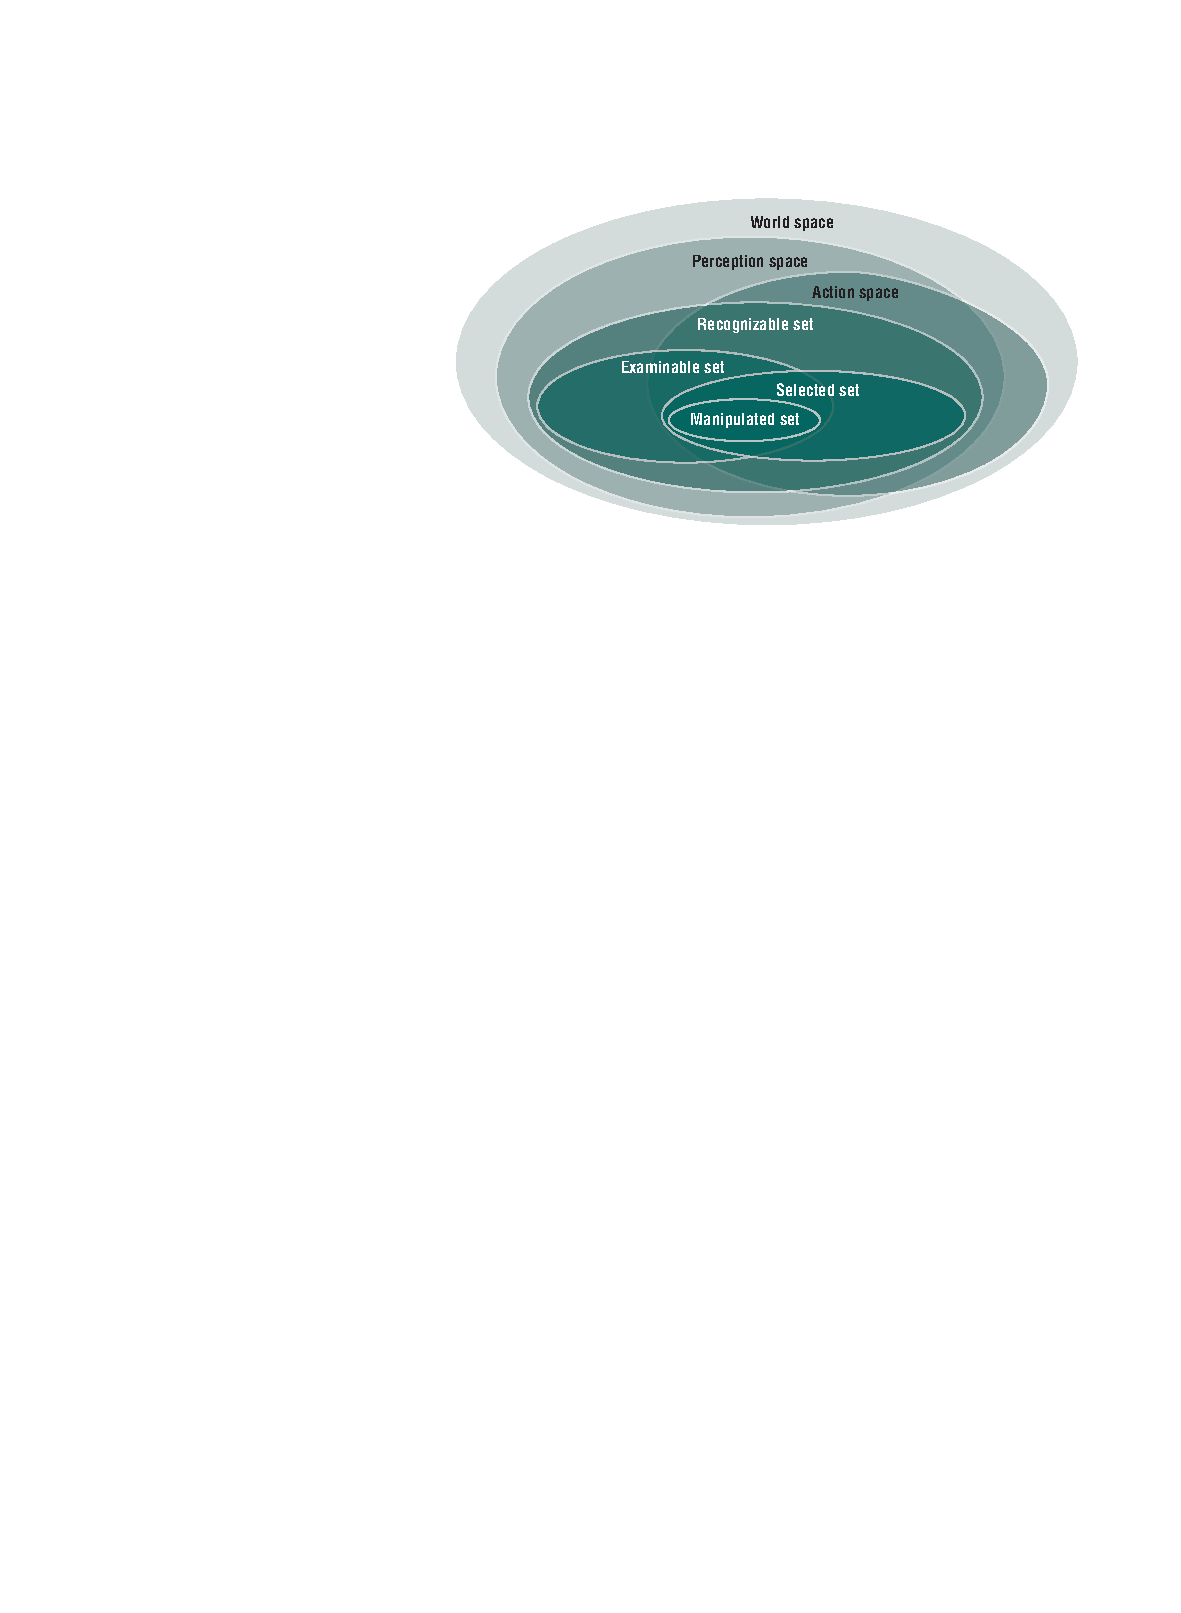
\includegraphics[width=0.7\linewidth]{gfx/Chapter3/ssm_sets}
	\caption{A situative space model (SSM). The spaces represent presence and approximate spatial relationship among physical and virtual objects with respect to what a specific human agent can perceive (perception space) and manipulate (action space) at a given moment in time. Whether objects are perceivable and manipulable depends on their relations to the human agent in all available interaction modalities (for example, vision, touch, and audio).\cite{pederson2011situative}}
	\label{fig:req_ssm_sets}
\end{figure}

As described in the definitions above, in order to correctly classify objects, they need to be augmented with the following parameters: \emph{PERCEPTION\_DISTANCE}, \emph{RECOGNITION\_DISTANCE}, \emph{EXAMINATION\_DISTANCE} and \emph{ACTION\_DISTANCE}. Normally, they should be given meaningful default values, therefore configuring them should not be a mandatory step. Even so, some objects might need adjusted values, so the possibility should be given to the system designer.
% section requirements (end)
%************************************************
\section{Architecture} % (fold)
\label{sec:architecture}
%************************************************
In this section we will describe the high level components we have developed to accommodate the requirements described in Section \ref{sec:requirements}. To empower the system designer to set up a simulation we need a \emph{Simulation Designer}. Using the simulation designer, the system designer is able to create a \emph{Configured Environment Model}, where all the objects of interest for the simulation have been identified and configured. The \emph{Simulation Runtime} loads a configured environment model and enables the simulation user to control an \emph{Avatar} in order to interact with the environment. As the agent interacts with the environment, the \emph{Context Manager} monitors the agent's position and visual spectrum, delegating the classification of objects around the user to the \emph{SSM Classifier}. The \emph{SSM Sets} can be visualized in the \emph{Context Client} and can be accessed through the \emph{API}.\\

For a better overview, the proposed architecture is illustrated in Figure \ref{fig:initial_architecture}.

\begin{figure}[H]
	\centering
	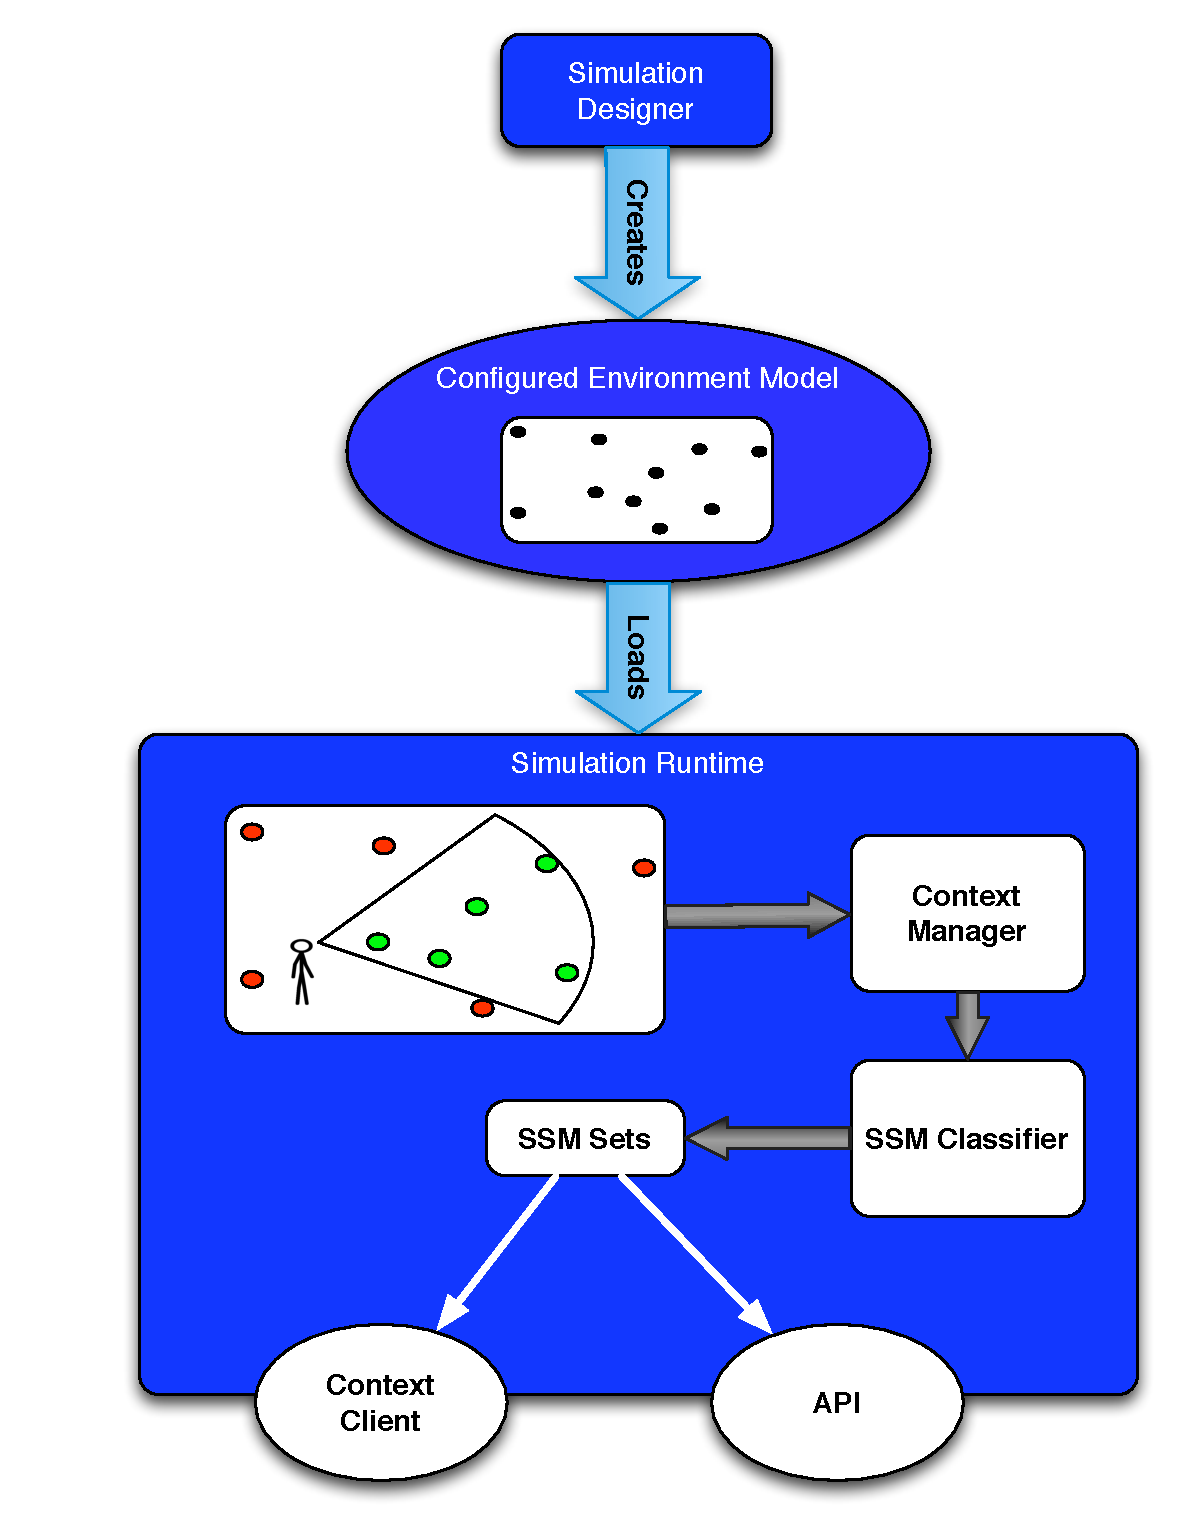
\includegraphics[width=0.8\linewidth]{gfx/Chapter3/initial_architecture}
	\caption{EgoSim Architecture Diagram}
	\label{fig:initial_architecture}
\end{figure}
% Describe the big picture in words and using a picture as well! Describe the main components imposed by this architecture: 3D modelling (to represent the space), rendering and movement control to build the simulated environment, categorization algorithms AND programming API (including the ContextClient).\\

% In the remaining of this chapter good deep into details about why I've chose certain technologies for each component; put each discussion in its own section! To better argue, present several technologies that could fit the same requirements and argue objectively about the the reasons I've made certain choices. I should refer back to arguments in the related work!

% section architecture (end)

% \begin{enumerate}
% 	\item Follow a modular design to implement the core of the framework as a set of decoupled components:
% 		\begin{itemize}
% 			\item The \emph{Data Model}. This represents the contextual entities and the relationship between them that the simulator will monitor, briefly detailed in Section \ref{sec:data_model}.
% 			\item The \emph{World Model}. Represents the current status of the simulated environment (e.g. position of the agent, status of a certain switch etc.). The structure of the entities in this model have been defined in the Data Model.
% 			\item A universal communication protocol to access the core. It needs to be universal so that other components, can easily be developed and integrated.
% 			\item Query and modify API of information in the World Model. To make the integration between the core of the framework and the other modules, these APIs will need to provide a complete set of methods.
% 		\end{itemize}
% 	\item Evaluate the framework:
% 		\begin{itemize}
% 			\item Implement a module to modify the state of the simulated environment (DummySim). This comprises of manipulating the agent's parameters and performing actions like picking up an item, touching a screen etc. The purpose of this module is to evaluate the modify API of the core. It also servers as a tool to modify the environment which is a required input for the SSM model to be evaluated.
% 			\item Implement the \emph{SSM Model}. Using the current World Model's query API, retrieve the current set of contextual data and apply the rules defined in the SSM. This component will actively monitor the current status of the simulator, having as a result an up to date collection of SSM entity sets: world space, perception space, recognizable set, examinable set, action space, selected set and manipulated set. This evaluation will be considered successful if the results are similar to the results obtained in the initial evaluation of the SSM described in \cite{pederson2011situative}.
% 		\end{itemize}
% \end{enumerate}


% In order to allow the user of the simulator to easily interact with the simulated environment, the visualization is really important. Projects that simulate real world scenarios, employ game alike solution providing complex graphics and interaction between the user of the simulator and the simulated world.\\

% This work represents initial research for this egocentric simulator. Therefore, my main focus is on the framework's core. But, I will invest time in researching existing solutions, either 2D or 3D; if I will document the suitable frameworks with high potential. This is nice-to-have. I don't want to set it as a goal of this project, rather talk about it as future work.

% \subsection{Data Model}\label{sec:data_model}
% The data model is aimed at defining the supported entities and the relationships between them. In this work the aim is to support physical objects, virtual objects and mediators.\\

% The agent represents a virtual character that can freely moved around in the environment. Beside the position the of the agent, the user can also control more complex parameters of the agent like orientation (affects field of vision), sitting down / standing, hands orientation etc. The agent will be also be able to carry out a certain set of actions like picking objects up, putting objects down etc.\\

% Physical objects will be described as entities with a certain set of properties (location, weight etc.). Entity composition will be supported to some extend: place objects on top of each other (i.e. a stapler on a table), a mobile phone in the backpack worn by the agent.\\

% This section created a brief overview of the supported entity types and relationships. They will be described in details in Chapter \ref{ch:design}.